\documentclass[xcolor={x11names,svgnames}]{beamer}

%\includeonlyframes{red}

\usepackage[french]{babel}
\usepackage[T1]{fontenc}
\usepackage{cellspace}

\usepackage{amsmath}
\usepackage{amsfonts}
\usepackage{tikz}
\usepackage{xspace}
%\usepackage[absolute,overlay]{textpos}
\usepackage[normalem]{ulem}
\usepackage{minted}

%\usepackage{eurosym}
\usepackage{marvosym}
\usepackage{pifont}
\usepackage{xcolor}

\newcommand{\bigO}[1]{\ensuremath{\mathcal{O}\left( #1 \right)} }

\newcommand{\red}{\alert}
\newcommand{\green}{\color{LimeGreen}}
\newcommand{\blue}{\color{cyan}}

% FORTIN
\newcommand{\mynote}[1]{\note<1>[item]{#1}}
\newcommand{\euro}{\EUR\xspace}

\usetikzlibrary{patterns}
\usetikzlibrary{snakes}
 \usetikzlibrary{arrows}
\usetikzlibrary{backgrounds}
\usetikzlibrary{shapes}
\usetikzlibrary{shadows}
\usetikzlibrary{calc}
\usetikzlibrary{decorations}
\usetikzlibrary{decorations.pathmorphing}
\usetikzlibrary{decorations.shapes}
\usetikzlibrary{decorations.markings}
\usetikzlibrary{positioning}

\definecolor{amethyst}{rgb}{0.6, 0.4, 0.8}
\definecolor{cyan}{rgb}{0,0.6796875,1}

\usecolortheme{rose}
\setbeamertemplate{footline}{}
\setbeamertemplate{navigation symbols}{}

\usepackage{fontspec}

\setsansfont{PalatinoSansLTPro}[
   Path = /home/charles/charles_work/fonts/PalatinoSans/, 
   Extension      = .otf,
   UprightFont    = *-Regular,
   BoldFont= *-Bold ,
   ItalicFont = *-Italic,
   BoldItalicFont = *-BoldIta
]

\author[C.~Bouillaguet]{Charles Bouillaguet \newline
  {\small (\texttt{charles.bouillaguet@lip6.fr})}}

\title{Cours 3 : (Un peu) d'algorithmique parallèle}
\date{2021-02-12}

\begin{document}




\begin{frame}[label=title]
  \titlepage
\end{frame}

\section{Généralités}

%%%%%%%%%%%%%%%%%%%%%%%%%%%%%%%%%%%%%%%%%%%%%%%%%%%%%%%%%%%%%%%%%%%%%%
\begin{frame}
\frametitle{Comment obtenir un programme parallèle efficace ?}

\begin{block}{Les grands principes}

\begin{itemize}
\item {\bf localité des données} : {\it répartir les données de sorte que
  chaque processeur dispose localement d'un maximum de données à traiter.}

\medskip

\item {\bf équilibrage de charge} ({\it load balancing}) : {\it attribuer au mieux les charges de
  calcul en fonction des caractéristiques de chaque processeur, afin
  de limiter les périodes d'inactivité.}

\medskip

\item {\bf recouvrement des communications par le calcul} : {\it éviter que les
    processeurs restent passifs pendant les phases de communications.}
\end{itemize}
\end{block}

\end{frame}


%%%%%%%%%%%%%%%%%%%%%%%%%%%%%%%%%%%%%%%%%%%%%%%%%%%%%%%%%%%%%%%%%%%%%%
\begin{frame}
\frametitle{\'Equilibrages de charge}


\begin{exampleblock}{Charge de calcul prédictible}

  \begin{itemize}
  \item[$\Rightarrow$] équilibrage de charge \textbf{statique}.
    
  \item Toutes les données nécessitent le même temps de calcul.

    $\rightarrow$ distribution par bloc, cyclique, \dots 
    
  \item Données régulières présentant des temps de calcul différents 

    $\rightarrow$ utilisation d'une fonction de coût $+$ distribution
    bloc, cyclique, \dots 

\end{itemize}
\end{exampleblock}

\medskip

\begin{alertblock}{Charge de calcul non prédictible}
  \begin{itemize}
   \item[$\Rightarrow$] équilibrage de charge \textbf{dynamique}
   \item modèle \sout{maître-esclave} patron-ouvrier
   \item modèle auto-régulé (\og vol de travail\fg)
   \end{itemize}
 \end{alertblock}


\end{frame}


%%%%%%%%%%%%%%%%%%%%%%%%%%%%%%%%%%%%%%%%%%%%%%%%%%%%%%%%%%%%%%%%%%%%%%
\begin{frame}
\frametitle{Modèle patron-ouvrier (maître-esclave)}


\begin{itemize} 
\item Le patron connaît les données et le travail à faire
\item Les ouvriers disponibles demandent du travail
\item Le patron des ordres de travail ou un ordre de fin

\begin{alertblock}{Limites}
\begin{itemize}
\item Si le patron doit charger toutes les données, il lui faut beaucoup de RAM
\item 2 envois de messages par tâche (A/R) $\longrightarrow$ grosse granularité
\item Trop d'ouvriers $\rightarrow$ le patron peut être un goulet d'étranglement
\end{itemize}
\end{alertblock}

\begin{exampleblock}{Avantages~:}
\begin{itemize}
\item l'équilibrage de charge, même avec matériel hétérogène (ou disponibilité/vitesse qui varie dans le temps)
\item \emph{checkpointing} assez facile (seulement le patron)
\end{itemize}
\end{exampleblock}

\end{itemize}

\end{frame}


%%%%%%%%%%%%%%%%%%%%%%%%%%%%%%%%%%%%%%%%%%%%%%%%%%%%%%%%%%%%%%%%%%%%%%
\begin{frame}
\frametitle{Modèle auto-régulé}

\begin{exampleblock}{Principe du \og vol de travail \fg~ ({\it work stealing})}

\begin{itemize} 
\item Chaque processeur gère sa propre liste de travaux à
  effectuer

  \begin{itemize}
  \item Répartition initiale équitable a priori
  \end{itemize}

\item Si la liste de travail d'un processeur est vide :
  \begin{itemize}
  \item Choisit une \emph{victime} (aléatoirement ?)
  \item \og Vole\fg une fraction (50\% ?) du travail restant à la victime
  \end{itemize}
\end{itemize}
\end{exampleblock}

\bigskip

\begin{itemize}
\item [+] Complètement symétrique
  \begin{itemize}
  \item Ni dieu ni maître \CircledA
  \end{itemize}
  
\item [+] tous les processeurs participent au calcul
  \begin{itemize}
  \item Pas de \sout{parasite} patron qui se tourne les pouces
    
  \end{itemize}
\item [--] pas facile de détecter qu'il n'y a plus de travail
\item [--] difficulté de programmation
\item [--] difficulté de \emph{checkpointing}
\end{itemize}

\end{frame}



%%%%%%%%%%%%%%%%%%%%%%%%%%%%%%%%%%%%%%%%%%%%%%%%%%%%%%%%%%%%%%%%%%%%%

\begin{frame}[fragile]
\frametitle{Parallélisme de données}


\begin{block}{Exemple classique : \emph{map}}
\begin{minted}{C}
for (int i = 0; i < n; i++)
    B[i] = f(A[i], i)
\end{minted}
\end{block}

\bigskip

\begin{itemize}
\item Pas besoin de communication / synchronisation !
\item Répartition des données ?
\item Équilibrage de charge
\end{itemize}
\end{frame}

%%%%%%%%%%%%%%%%%%%%%%%%%%%%%%%%%%%%%%%%%%%%%%%%%%%%%%%%%%%%%%%%%

\section{Distribution de données}

\begin{frame}
\frametitle{Répartition 1D}

Par blocs :

\medskip

\begin{tikzpicture}
  \filldraw[fill=red]    (0, 0) rectangle  +(1,1);
  \filldraw[fill=orange] (1, 0) rectangle  +(1,1);
  \filldraw[fill=yellow] (2, 0) rectangle  +(1,1);
  \filldraw[fill=green]  (3, 0) rectangle  +(1,1);
  \filldraw[fill=cyan]   (4, 0) rectangle  +(1,1);
  \filldraw[fill=blue]   (5, 0) rectangle  +(1,1);
  \filldraw[fill=magenta] (6, 0) rectangle  +(1,1);
  \filldraw[fill=violet] (7, 0) rectangle +(1,1);
  \filldraw[fill=lightgray] (8, 0) rectangle +(1,1);
  \filldraw[fill=darkgray] (9, 0) rectangle +(1,1);
  
  \draw[thick] (0, 0) rectangle (10, 1);
  \foreach \i in {0.2, 0.4, ..., 9.8}
  \draw (\i, 0) -- +(0, 1);
\end{tikzpicture}

\begin{itemize}
\item Le plus simple !
\item Favorisé par MPI
\end{itemize}

\vspace{1cm}

Cyclique :

\medskip

\begin{tikzpicture}
  \foreach \i in {0, 2, 4, 6, 8} {
    \filldraw[fill=red]    (\i, 0) rectangle  +(0.2,1);
    \filldraw[fill=orange]    (\i + 0.2, 0) rectangle  +(0.2,1);
    \filldraw[fill=yellow]    (\i + 0.4, 0) rectangle  +(0.2,1);
    \filldraw[fill=green]    (\i + 0.6, 0) rectangle  +(0.2,1);
    \filldraw[fill=cyan]    (\i + 0.8, 0) rectangle  +(0.2,1);
    \filldraw[fill=blue]    (\i + 1, 0) rectangle  +(0.2,1);
    \filldraw[fill=magenta]    (\i + 1.2, 0) rectangle  +(0.2,1);
    \filldraw[fill=violet]    (\i + 1.4, 0) rectangle  +(0.2,1);
    \filldraw[fill=lightgray]    (\i + 1.6, 0) rectangle  +(0.2,1);
    \filldraw[fill=darkgray]    (\i + 1.8, 0) rectangle  +(0.2,1);
  }
  % \filldraw[fill=red]    (0, 0) rectangle  +(1,1);
  % \filldraw[fill=orange] (1, 0) rectangle  +(1,1);
  % \filldraw[fill=yellow] (2, 0) rectangle  +(1,1);
  % \filldraw[fill=green]  (3, 0) rectangle  +(1,1);
  % \filldraw[fill=cyan]   (4, 0) rectangle  +(1,1);
  % \filldraw[fill=blue]   (5, 0) rectangle  +(1,1);
  % \filldraw[fill=magenta] (6, 0) rectangle  +(1,1);
  % \filldraw[fill=violet] (7, 0) rectangle +(1,1);
  % \filldraw[fill=lightgray] (8, 0) rectangle +(1,1);
  % \filldraw[fill=darkgray] (9, 0) rectangle +(1,1);
  
  \draw[thick] (0, 0) rectangle (10, 1);
  \foreach \i in {0.2, 0.4, ..., 9.8}
  \draw (\i, 0) -- +(0, 1);
\end{tikzpicture}

\begin{itemize}
\item Améliore parfois l'équilibrage de charge.
\item Possible aussi avec MPI (\texttt{MPI\_Type\_vector}...)
\end{itemize}
\end{frame}

%%%%%%%%%%%%%%%%%%%%%%%%%%%%%%%%%%%%%%%%%%%%%%%%%%%%

\begin{frame}
\frametitle{Répartition 1D (de données 2D)}

Par blocs :

\medskip

\begin{tikzpicture}[scale=0.5]
  \filldraw[fill=red]    (0, 0) rectangle  +(12,3);
  \filldraw[fill=orange] (0, 3) rectangle  +(12,3);
  \filldraw[fill=green] (0, 6) rectangle  +(12,3);
  \filldraw[fill=cyan]  (0, 9) rectangle  +(12,3);
  
  \draw[thick] (0, 0) rectangle (12, 12);
  \foreach \i in {1, 2, ..., 11} {
    \draw (\i, 0) -- +(0, 12);
    \draw (0, \i) -- +(12, 0);
  }
\end{tikzpicture}
\end{frame}


%%%%%%%%%%%%%%%%%%%%%%%%%%%%%%%%%%%%%%%%%%%%%%%%%%%%

\begin{frame}
\frametitle{Répartition 1D (de données 2D)}

Cyclique :

\medskip

\begin{tikzpicture}[scale=0.5]
  \foreach \i in {0, 4, 8} {
    \filldraw[fill=red]    (0, \i) rectangle  +(12,1);
    \filldraw[fill=orange] (0, 1+\i) rectangle  +(12,1);
    \filldraw[fill=green] (0, 2+\i) rectangle  +(12,1);
    \filldraw[fill=cyan]  (0, 3+\i) rectangle  +(12,1);
  }
  \draw[thick] (0, 0) rectangle (12, 12);
  \foreach \i in {1, 2, ..., 11} {
    \draw (\i, 0) -- +(0, 12);
    \draw (0, \i) -- +(12, 0);
  }
\end{tikzpicture}
\end{frame}

%%%%%%%%%%%%%%%%%%%%%%%%%%%%%%%%

\begin{frame}
\frametitle{Répartition 2D (de données 2D)}

Par blocs :

\medskip

\begin{tikzpicture}[scale=0.5]
  \filldraw[fill=red]    (0, 0) rectangle  +(6, 6);
  \filldraw[fill=orange] (0, 6) rectangle  +(6,6);
  \filldraw[fill=green] (6, 0) rectangle  +(6,6);
  \filldraw[fill=cyan]  (6, 6) rectangle  +(6,6);

  \draw[thick] (0, 0) rectangle (12, 12);
  \foreach \i in {1, 2, ..., 11} {
    \draw (\i, 0) -- +(0, 12);
    \draw (0, \i) -- +(12, 0);
  }
\end{tikzpicture}
\end{frame}

%%%%%%%%%%

\begin{frame}
\frametitle{Répartition 2D (de données 2D)}

Cyclique :

\medskip

\begin{tikzpicture}[scale=0.5]
  \foreach \i in {0, 2, 4, 6, 8, 10} {
    \foreach \j in {0, 2, 4, 6, 8, 10} {
      \filldraw[fill=red]    (\i, \j) rectangle  +(1, 1);
      \filldraw[fill=orange] (\i, 1+\j) rectangle  +(1,1);
      \filldraw[fill=green] (\i+1, \j) rectangle  +(1,1);
      \filldraw[fill=cyan]  (\i+1, 1+\j) rectangle  +(1,1);
    }
  }
  \draw[thick] (0, 0) rectangle (12, 12);
  \foreach \i in {1, 2, ..., 11} {
    \draw (\i, 0) -- +(0, 12);
    \draw (0, \i) -- +(12, 0);
  }
\end{tikzpicture}
\end{frame}

%%%%%%%%%%%%%%%%%%%%%%%%

\begin{frame}
\frametitle{Répartition 1D (de données 3D)}

\centering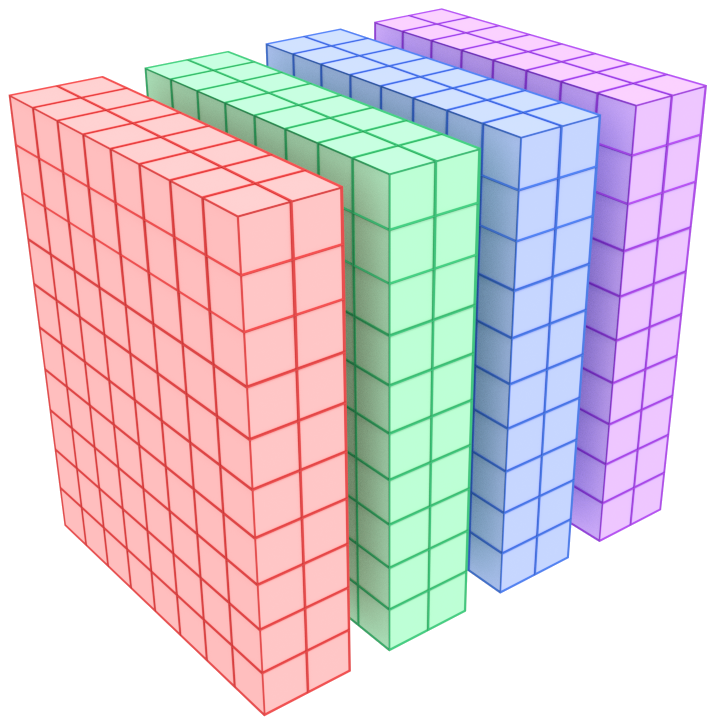
\includegraphics[height=8cm]{slabs.png}

\end{frame}

%%%%%%%%%%%%%%%%%%%%%%%%

\begin{frame}
\frametitle{Répartition 2D (de données 3D)}

\centering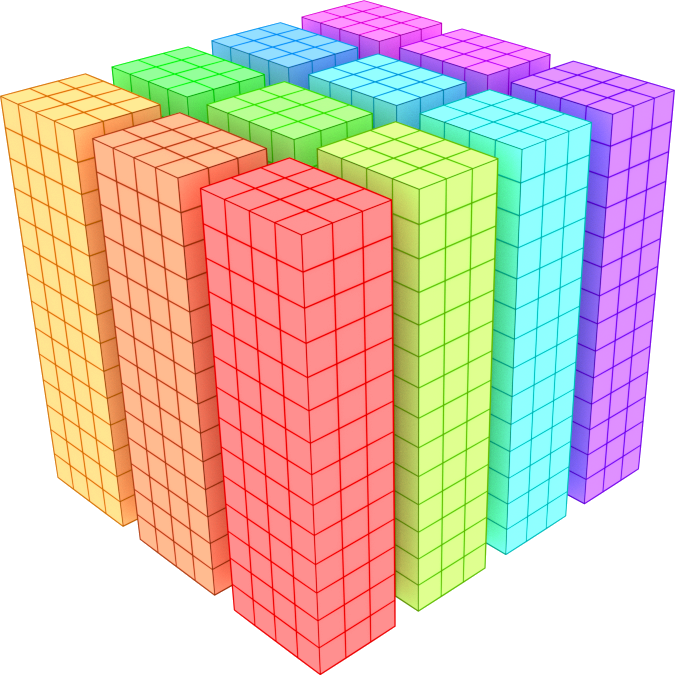
\includegraphics[height=8cm]{pencils.png}

\end{frame}

%%%%%%%%%%%%%%%%%%%%%%%%%

\section{Algos et coût des opérations collectives}

\begin{frame}[fragile]
\frametitle{Parallélisme de données}


\begin{block}{Exemple classique : \emph{reduce}}
\begin{minted}{C}
sum = 0
for (int i = 0; i < n; i++)
    sum = sum + A[i]
\end{minted}
\end{block}

\bigskip

\begin{itemize}
\item Mémoire distribuée $\rightarrow$ communications
\item Algorithme \og classique\fg en arbre.
\end{itemize}
\end{frame}

%%%%%%%%%%%%%%%%%%%%%%%%%%%%%%%%%%%%%%%%%%%%%%%%%%%%%%%%%%%%%%%%

\begin{frame}
\frametitle{Algorithme (mémoire partagée) pour \texttt{reduce}}

\begin{tikzpicture}
  \filldraw[fill=red]    (0, 0) rectangle  +(1,1);
  \filldraw[fill=orange] (1, 0) rectangle  +(1,1);
  \filldraw[fill=yellow] (2, 0) rectangle  +(1,1);
  \filldraw[fill=green]  (3, 0) rectangle  +(1,1);
  \filldraw[fill=cyan]   (4, 0) rectangle  +(1,1);
  \filldraw[fill=blue]   (5, 0) rectangle  +(1,1);
  \filldraw[fill=magenta] (6, 0) rectangle  +(1,1);
  \filldraw[fill=violet] (7, 0) rectangle +(1,1);
  \filldraw[fill=lightgray] (8, 0) rectangle +(1,1);
  \filldraw[fill=darkgray] (9, 0) rectangle +(1,1);
  
  \draw[thick] (0, 0) rectangle (10, 1);
  \foreach \i in {0.2, 0.4, ..., 9.8}
  \draw (\i, 0) -- +(0, 1);
\end{tikzpicture}

\bigskip

\begin{enumerate}
\item Tableau \texttt{Scratch} de taille $p$.
\item $P_i$ fait : $\texttt{Scratch[i]} \gets $ somme de \emph{ses} donnée.
\item \alert{Barrière}
\item $P_0$ calcule la somme de \texttt{Scratch} puis l'écrit dans \texttt{sum}
\item \alert{Barrière}
\end{enumerate}


\begin{align*}
  T &= \frac{n}{p} + p \\
    &\geq 2 \sqrt{n} & \text{(optimal atteint avec $\sqrt{n}$ processeurs)}
\end{align*}
\end{frame}

%%%%%%%%%%%%%%%%%%%%%%%%%%%%%%%%%%%%%%%%% 

%%%%%%%%%%%%%%%%%%%%%%%%%%%%%%%%%%%%%%%%%%%%%%%%%%%%%%%%%%%%%%%%

\begin{frame}
\frametitle{Algorithme (mémoire partagée) pour \texttt{reduce}}

\begin{tikzpicture}
  \filldraw[fill=red]    (0, 0) rectangle  +(1,1);
  \filldraw[fill=orange] (1, 0) rectangle  +(1,1);
  \filldraw[fill=yellow] (2, 0) rectangle  +(1,1);
  \filldraw[fill=green]  (3, 0) rectangle  +(1,1);
  \filldraw[fill=cyan]   (4, 0) rectangle  +(1,1);
  \filldraw[fill=blue]   (5, 0) rectangle  +(1,1);
  \filldraw[fill=magenta] (6, 0) rectangle  +(1,1);
  \filldraw[fill=violet] (7, 0) rectangle +(1,1);
  \filldraw[fill=lightgray] (8, 0) rectangle +(1,1);
  \filldraw[fill=darkgray] (9, 0) rectangle +(1,1);
  
  \draw[thick] (0, 0) rectangle (10, 1);
  \foreach \i in {0.2, 0.4, ..., 9.8}
  \draw (\i, 0) -- +(0, 1);
\end{tikzpicture}

\bigskip

\begin{block}{$\texttt{reduce}(A, n):$}
  \begin{enumerate}
  \item Si $n = 1$, renvoyer $A[0]$.
  \item Allouer un tableau \texttt{Scratch} de taille $n/2$.
  \item Pour tout $0 \leq i < n/2$, faire (en parallèle):
    \begin{itemize}
    \item $\texttt{Scratch}[i] \gets A[2i] + A[2i+1]$.  
    \end{itemize}
    
  \item renvoyer : $\texttt{reduce}(\texttt{Scratch}, n/2)$.
  \end{enumerate}
\end{block}

\begin{align*}
  T &= \frac{2n}{p} + \log_2 p \\
    &\geq 1 + \log_2 p & \text{(optimal atteint avec $n/2$ processeurs)}
\end{align*}
\end{frame}


%%%%%%%%%%%%%%%%%%%%%%%%%%%%%%%%%%%%%%%%%%%%%%%%%%%%%%%%%%%%%%%%

\begin{frame}
\frametitle{Durée des communications ?}


\begin{block}{Envoi d'un message du rang $i$ au rang $j$}
  \[
    T = \alpha + n \times \beta
  \]
  
  \begin{itemize}
  \item $n =$ taille des données (bit)
  \item $\alpha =$ \alert{latence} (s)
  \item $\beta \approx$ \alert{débit} (s / bit).
  \end{itemize}
\end{block}

\medskip

$1 / \beta$ : bit / s (\alert{bande passante}).

\medskip

\begin{alertblock}{Modèle simplifié !}
\begin{itemize}
\item $T$ indépendant de $i$ et $j$ (topologie ?)
\item Indépendant des autres envois (congestion ?)
\end{itemize}
\end{alertblock}

\end{frame}

%%%%%%%%%%%%%%%%%%%%%%%%%%%%%%%%%%%%%%%%%%%%%%%%%%%%%%%%%%%%%%%%%


\begin{frame}[label=red]
  \frametitle{\texttt{reduce} : méthode de l'arbre binaire}
  \begin{center}
    \begin{tikzpicture}[level distance=10mm, xscale=0.66, yscale=0.75]
  \foreach \i in {0,1,2,3,4,5,6} {
    \draw[semitransparent,gray] (-7, -6+\i) node[text=black,left] {t=\i} -- +(14, 0);
  }

  \node {1}
    child { node at (0, -1) {2}
      child { node at (0,-1) {4}
        child {node at (0, -1) {8}}
        child {node  {9}}
      }
      child[missing]
      child {node  {5}
        child {node at (0, -2) {10}}
        child {node at (0, -1) {11}}
      }
    }
    child[missing]
    child[missing]
    child[missing]
     child { node {3}
      child {node at (0, -2) {6}
        child {node at (0, -1) {12} }
        child {node at (0, 0) {13} }
      }
      child[missing]
      child {node  at (0, -1) {7}
        child {node at (0, -2) {14}}
        child {node at (0, -1) {15} }
      }
    }
;
\end{tikzpicture}
\end{center}

\begin{itemize}
\item Contribution de $2^h - 1$ reçue par 1 après $2(h-1)$ messages successifs
\item[$\Rightarrow$] $T \geq 2 \alpha (\lceil \log_2 P \rceil - 1)$
\end{itemize}
\end{frame}

%%%%%%%%%%%%%%

\begin{frame}
  \frametitle{\texttt{reduce} : méthode de l'arbre binomial}
  
  \begin{center}
    \begin{tikzpicture}[level distance=10mm, xscale=0.66, yscale=0.75]
  \foreach \i in {0,1,2,3,4} {
    \draw[semitransparent,gray] (-9, -4+\i) node[text=black,left] {t=\i} -- +(15, 0);
  }

  \node {0}
    child { node {8}
      child { node {12}
        child {node {14}
          child {node {15}}
        }
        child {node at (0, -1) {13}}
      }
      child[missing]
      child {node at (0,-1) {10}
        child {node {11}}
      }
      child {node at (0,-2) {9} }
    }
    child[missing]
    child[missing]
    child { node at (0, -1) {4}
      child {node {6}
        child {node {7} }
      }
      child {node at (0, -1) {5} }
    }
    child[missing]
    child { node at (0, -2) {2}
      child {node {3}}
    }
    child[missing]
    child { node at (0, -3) {1} }
;
\end{tikzpicture}
\end{center}

\begin{itemize}
\item Toutes les contributions reçues après $h$ envois successifs.
\item[$\Rightarrow$] $T \geq \alpha h$.
\end{itemize}

\bigskip

\begin{exampleblock}{\texttt{reduce}}
  $T = $ envoi de $\lceil \log_2 P \rceil$ messages de taille 1 $= \lceil \log_2 P \rceil \alpha$
\end{exampleblock}
\end{frame}

%%%%%%%%%%%%%%%%%%%%%%%%%%%%%%%%%%%%%%%%%%%%%%%%%%%%%%%%%%%%%%%%%

\begin{frame}[fragile]
\frametitle{Retour sur MPI : Gather / Scatter / Reduce}

%\setminted[C]{fontsize=\footnot}
\begin{minted}[fontsize=\footnotesize]{C}
int MPI_Gather(void* sendbuf, int sendcount, MPI_Datatype sendtype,
               void* recvbuf, int recvcount, MPI_Datatype recvtype,
               int root, MPI_Comm comm);
int MPI_Scatter(void* sendbuf, int sendcount, MPI_Datatype sendtype,
                void* recvbuf, int recvcount, MPI_Datatype recvtype,
                int root, MPI_Comm comm);
\end{minted}

\bigskip

\begin{center}
\begin{tikzpicture}[scale=0.5, >=latex]

  \node at (-1.5, 5.5) {root};
  
%%%%%%%%%%%% Scatter / Gather
  \begin{scope}
    \foreach \i in {0,1,...,6} {
      \draw[thick] (\i, 0) -- +(0, 6);
      \draw[thick] (0, \i) -- +(6, 0);
    }
    \foreach \i in {0,1,...,5}
    \node at (\i+0.5,  5.5) {$x_\i$};
  \end{scope}

\draw[ultra thick,->] (7, 4) -- node[above] {Scatter} (11, 4);
\draw[ultra thick,<-] (7, 2) -- node[below] {Gather} (11, 2);

\begin{scope}[xshift=12cm]
  \foreach \i in {0,1,...,6} {
    \draw[thick] (\i, 0) -- +(0, 6);
    \draw[thick] (0, \i) -- +(6, 0);
  }
  \foreach \i in {0,1,...,5}
    \node at (0.5, 5.5-\i) {$x_\i$};
\end{scope}
\end{tikzpicture}
\end{center}
\end{frame}


%%%%%%%%%%%%%%%%%%%%%%%%%%%%%%%%%%%%%%%%%%%%%%%%%%%%%%%%%%%%%%%%%%%%%%%%%%%%

\begin{frame}
\frametitle{Borne inférieure pour Scatter/Gather}

\begin{center}
\begin{tikzpicture}[scale=0.5, >=latex]

  \node at (-1.5, 5.5) {root};
  
%%%%%%%%%%%% Scatter / Gather
  \begin{scope}
    \foreach \i in {0,1,...,6} {
      \draw[thick] (\i, 0) -- +(0, 6);
      \draw[thick] (0, \i) -- +(6, 0);
    }
    \foreach \i in {0,1,...,5}
    \node at (\i+0.5,  5.5) {$x_\i$};
  \end{scope}

\draw[ultra thick,->] (7, 4) -- node[above] {Scatter} (11, 4);
\draw[ultra thick,<-] (7, 2) -- node[below] {Gather} (11, 2);

\begin{scope}[xshift=12cm]
  \foreach \i in {0,1,...,6} {
    \draw[thick] (\i, 0) -- +(0, 6);
    \draw[thick] (0, \i) -- +(6, 0);
  }
  \foreach \i in {0,1,...,5}
    \node at (0.5, 5.5-\i) {$x_\i$};
\end{scope}
\end{tikzpicture}
\end{center}

\begin{alertblock}{Sont inévitables...}
\begin{enumerate}
\item $(p-1) \frac{n}{p}$ données doivent sortir (resp. entrer) de \texttt{root}.
  \begin{itemize}
  \item $T \geq (p-1) \frac{n}{p} \beta$
  \end{itemize}
\item Atteindre tout le monde.
  \begin{itemize}
  \item $\log_2 p$ messages successifs (\og \textbf{épidémie} \fg)
  \end{itemize}
\item[\alert{$\Rightarrow$}] $T \geq \lceil \log_2 p \rceil \alpha + (p-1) \frac{n}{p} \beta$
\end{enumerate}

\end{alertblock}
\end{frame}

%%%%%%%%%%%%%%%%%%%%%%%%%%%%%%%%%%%%%%%%%%%%%%%%%%%%%%%%%%%%%%%%%%%%%%%%%%%%%%

\begin{frame}
  \frametitle{Méthode de l'arbre binomial}
  
  \begin{center}
    \begin{tikzpicture}[level distance=10mm, xscale=0.66, yscale=0.75]
  \foreach \i in {0,1,2,3,4} {
    \draw[semitransparent,gray] (-9, -\i) node[text=black,left] {t=\i} -- +(15, 0);
  }

  \node {$B_4$}
    child { node {$B_3$}
      child { node {$B_2$}
        child {node {$B_1$}
          child {node {$B_0$}}
        }
        child {node at (0, -1) {$B_0$}}
      }
      child[missing]
      child {node at (0,-1) {$B_1$}
        child {node {$B_0$}}
      }
      child {node at (0,-2) {$B_0$} }
    }
    child[missing]
    child[missing]
    child { node at (0, -1) {$B_2$}
      child {node {$B_1$}
        child {node {$B_0$} }
      }
      child {node at (0, -1) {$B_0$} }
    }
    child[missing]
    child { node at (0, -2) {$B_1$}
      child {node {$B_0$}}
    }
    child[missing]
    child { node at (0, -3) {$B_0$} }
;
\end{tikzpicture}
\end{center}

\begin{itemize}
\item Tous les $B_i$ sont contactés en même temps
\item Chaque $B_i$ reçoit $2^i \frac{n}{p}$ données.
\end{itemize}

\bigskip

\begin{exampleblock}{\texttt{Scatter/Gather}}
  ~
  \vspace{-0.7cm}
  \begin{align*}
    T &= \text{message de taille 1 $+ \dots +$ message de taille $n/2$} \\
      &= \alpha  \lceil\log_2 p\rceil + \left(p -1 \right)  \frac{n}{p} \beta \qquad \text{\alert{(optimal)}}
  \end{align*}
\end{exampleblock}
\end{frame}

%%%%%%%%%%%%%%%%%%%%%%%%%%%%%%%%%%%%%%%%%%%%%%%%%%%

\begin{frame}[fragile]
\frametitle{MPI : AllGather}

\begin{minted}[fontsize=\footnotesize]{C}
int MPI_Allgather(void* sendbuf, int sendcount, MPI_Datatype sendtype,
                  void* recvbuf, int recvcount, MPI_Datatype recvtype, 
                  MPI_Comm comm);
\end{minted}

\bigskip

\begin{center}
\begin{tikzpicture}[scale=0.5, >=latex]
  \begin{scope}
    \foreach \i in {0,1,...,6} {
      \draw[thick] (\i, 0) -- +(0, 6);
      \draw[thick] (0, \i) -- +(6, 0);
    }
    \foreach \i in {0,1,...,5}
    \node at (0.5,  5.5-\i) {$x_\i$};
  \end{scope}

\draw[ultra thick,->] (7, 3) -- node[above] {AllGather} (11, 3);

\begin{scope}[xshift=12cm]
  \foreach \i in {0,1,...,6} {
    \draw[thick] (\i, 0) -- +(0, 6);
    \draw[thick] (0, \i) -- +(6, 0);
  }
  \foreach \i in {0,1,...,5}
  \foreach \j in {0,1,...,5}
  \node at (\i+0.5, \j+0.5) {$x_\i$};
\end{scope}
\end{tikzpicture}
\end{center}
\end{frame}

%%%%%%%%%%%%%%%%%%%%%%%%%%%%

\begin{frame}
\frametitle{AllGather : algorithme de l'anneau}


\begin{columns}
  \begin{column}{6cm}
\begin{tikzpicture}[>=latex, scale=0.9]

  \foreach \i in {0,1,...,11} {
    \draw (\i*30:3cm) node (P\i) {$P_{\i}$};
  }
  \draw[->] (P0) edge[bend right] (P1);
  \draw[->] (P1) edge[bend right] (P2);
  \draw[->] (P2) edge[bend right] (P3);
  \draw[->] (P3) edge[bend right] (P4);
  \draw[->] (P4) edge[bend right] (P5);
  \draw[->] (P5) edge[bend right] (P6);
  \draw[->] (P6) edge[bend right] (P7);
  \draw[->] (P7) edge[bend right] (P8);
  \draw[->] (P8) edge[bend right] (P9);
  \draw[->] (P9) edge[bend right] (P10);
  \draw[->] (P10) edge[bend right] (P11);
  \draw[->] (P11) edge[bend right] (P0);

\end{tikzpicture}
\end{column}
\begin{column}{5cm}
  \begin{block}{algorithme}
    \begin{itemize}
    \item Phase 0 : \\ envoie \og ses\fg données
    \item Phase $i+1$ : \\ envoie msg reçu phase $i$
    \end{itemize}
  \end{block}

  \begin{exampleblock}{Analyse}
  \begin{itemize}
  \item 1 msg = $n/p$ données
  \item 1 phase = $p$ messages $//$
  \item AllGather = $p-1$ phases
  \item[\alert{$\Rightarrow$}] $T = (p-1)(\alpha + \frac{n}{p}\beta)$
  \end{itemize}

\end{exampleblock}
\end{column}
\end{columns}
\end{frame}

%%%%%%%%%%%%%%%%%%%%%%%%%%%%%%%%%%%%%%%%%%%%%%%%%%%%

\begin{frame}
\frametitle{AllGather : algorithme du doublage récursif}

\begin{center}
  \begin{tikzpicture}[>=latex, scale=0.66]
    \path[red, use as bounding box] (-0.5, 0.5) rectangle (14.5, -6);
\foreach \i in {0,1,2,3,4,5,6,7}
  \draw (2*\i, 0) node [draw,shape=circle] (N\i) {\i};

%\node at (-0.5, -0.75) {$i=0$};
\foreach \a / \b in {0/1, 2/3, 4/5, 6/7}
  \draw[<->,transform canvas={yshift=-0.5cm}] (N\a) edge [bend right=45] (N\b);

%\node at (-0.5, -2) {$i=1$};
\foreach \a / \b in {0/2, 1/3, 4/6, 5/7}
  \draw[<->,transform canvas={yshift=-1.5cm}] (N\a) edge[bend right=45] (N\b);

%\node at (-0.5, -4) {$i=2$};
\foreach \a / \b in {0/4, 1/5, 2/6, 3/7}
  \draw[<->,transform canvas={yshift=-3cm}] (N\a) to[bend right=35] (N\b);
\end{tikzpicture}
\end{center}

\bigskip

\[
T = \alpha \log_2 p + (p-1) \frac{n}{p} \beta \qquad \text{\alert{(optimal)}}
\]
\end{frame}

%%%%%%%%%%%%%%%%%%%%%%%%%%%%%%%%%%%%%%%%%%%%%%%%%%%%

\begin{frame}[fragile]
\frametitle{MPI : Broadcast}

\begin{minted}[fontsize=\footnotesize]{C}
int MPI_Bcast(void* buffer, int count, MPI_Datatype datatype, 
              int root, MPI_Comm comm);
\end{minted}


\begin{center}
\begin{tikzpicture}[scale=0.5, >=latex]
%Bcast
\begin{scope}
  \begin{scope}
    \foreach \i in {0,1,...,6} {
      \draw[thick] (\i, 0) -- +(0, 6);
      \draw[thick] (0, \i) -- +(6, 0);
    }
    \node at (0.5, 5.5) {$x$};
  \end{scope}

\draw[ultra thick,->] (7, 3) -- node[above] {Broadcast} (11, 3);

\begin{scope}[xshift=12cm]
  \foreach \i in {0,1,...,6} {
    \draw[thick] (\i, 0) -- +(0, 6);
    \draw[thick] (0, \i) -- +(6, 0);
  }
  \foreach \i in {0,1,...,5}
    \node at (0.5, 5.5-\i) {$x$};
\end{scope}
\end{scope}
\end{tikzpicture}
\end{center}

\begin{alertblock}{Borne inférieure}
\begin{enumerate}
\item $n$ données doivent sortir de \texttt{root}.
\item Atteindre tout le monde.
\item[\alert{$\Rightarrow$}] $T \geq \lceil \log_2 p \rceil \alpha + n \beta$
\end{enumerate}
\end{alertblock}
\end{frame}

%%%%%%%%%%%%%%%%%%%%%

\begin{frame}
\frametitle{Algorithmes pour Broadcast}

\begin{block}{Arbre binomial}
  \begin{itemize}
  \item $T = \lceil \log_2 p \rceil (\alpha + n \beta)$
  \item Terme \og débit\fg sous-optimal
  \item (mauvais pour grands messages)
  \end{itemize}
\end{block}

\bigskip

\begin{block}{Van de Geijn}
  \begin{itemize}
  \item Broadcast = Scatter puis AllGather (2rec)
  \item $T = \alert{2}  (\log_2 p) \alpha +  \alert{2} \left(1 - \frac{1}{p}\right) n \beta$
  \item[$\rightarrow$] $2\times$ borne inf'
  \end{itemize}
\end{block}
\end{frame}

%%%%%%%%%%%%%%%%%%%%%%%%%%%%%%%%%%%%%

\section{Prefix-Sum}

\begin{frame}[fragile]
\frametitle{Parallélisme de données}


\begin{block}{Exemple classique : \emph{prefix-sum} (``scan'') (en place)}
\begin{minted}{C}
for (int i = 1; i < n; i++)
    A[i] = A[i] + A[i - 1];
\end{minted}
\end{block}

\bigskip

\begin{itemize}
\item \textbf{Dépendance de données}
\item Chaque itération a besoin du résultat de la précédente...
\item Changer l'algorithme   
\end{itemize}
\end{frame}

%%%%%%%%%%%%%%%%%%%%%%%%%%%%%%%%%%%%%%%%%%%%%%%%%%%%%%%%%%%%%%%%

\begin{frame}[fragile]
\frametitle{\texttt{prefix-sum} : Cas de la mémoire partagée}


\begin{block}{Exemple classique : \emph{prefix-sum} (en place)}
\begin{minted}[fontsize=\small]{C}
double *B;

void prefix_sum(double * A, int n)
{
    if (n < 2)
        return;
    for (int i = 0; i < n / 2; i++)
        B[i] = A[2 * i] + A[2 * i + 1];
    prefix_sum(B, k);
    for (int i = 1; i < n; i += 2) {
          A[i] = B[i / 2];
          A[i + 1] = B[i / 2] + A[i + 1];
    }
}
\end{minted}
\end{block}


\end{frame}


%%%%%%%%%%%%%%%%%%%%%%%%%%%%%%%%%%%%%%%%%%%%%%%%%%%%%%%%%%%%%%%%%

\begin{frame}
\frametitle{Algorithme MIMD-DM pour \texttt{prefix-sum}}

\begin{tikzpicture}
  \filldraw[fill=red]    (0, 0) rectangle  +(1,1);
  \filldraw[fill=orange] (1, 0) rectangle  +(1,1);
  \filldraw[fill=yellow] (2, 0) rectangle  +(1,1);
  \filldraw[fill=green]  (3, 0) rectangle  +(1,1);
  \filldraw[fill=cyan]   (4, 0) rectangle  +(1,1);
  \filldraw[fill=blue]   (5, 0) rectangle  +(1,1);
  \filldraw[fill=magenta] (6, 0) rectangle  +(1,1);
  \filldraw[fill=violet] (7, 0) rectangle +(1,1);
  \filldraw[fill=lightgray] (8, 0) rectangle +(1,1);
  \filldraw[fill=darkgray] (9, 0) rectangle +(1,1);
  
  \draw[thick] (0, 0) rectangle (10, 1);
  \foreach \i in {0.2, 0.4, ..., 9.8}
  \draw (\i, 0) -- +(0, 1);
\end{tikzpicture}

\bigskip

\begin{enumerate}
\item $P_i$ calcule la somme $S_i$ de \emph{ses} données. \hfill \alert{[local]}
\item Ils font (collectivement) $T \gets \texttt{prefix-sum}(S)$.
  \begin{itemize}
  \item \texttt{MPI\_Scan}
  \end{itemize}
\item[$\rightarrow$] $P_i$ obtient $T_i = $ somme des données des $P_j$ (pour $j<i$).
\item $P_i$ \texttt{prefix-sum} ses données en ajoutant $T_i$. \hfill \alert{[local]}
\end{enumerate}
\end{frame}

%%%%%%%%%%%%%%%%%%%%%%%%%%%%%%%%%%%%%%%%% 

\begin{frame}
  \frametitle{Rappel : \texttt{reduce} par la méthode de l'arbre binomial}
  
  \begin{center}
    \begin{tikzpicture}[level distance=10mm, xscale=0.66, yscale=0.75]
  \foreach \i in {0,1,2,3,4} {
    \draw[semitransparent,gray] (-9, -4+\i) node[text=black,left] {t=\i} -- +(15, 0);
  }

  \node {15}
    child { node {7}
      child { node {3}
        child {node {1}
          child {node {0}}
        }
        child {node at (0, -1) {2}}
      }
      child[missing]
      child {node at (0,-1) {5}
        child {node {4}}
      }
      child {node at (0,-2) {6} }
    }
    child[missing]
    child[missing]
    child { node at (0, -1) {11}
      child {node {9}
        child {node {8} }
      }
      child {node at (0, -1) {10} }
    }
    child[missing]
    child { node at (0, -2) {13}
      child {node {12}}
    }
    child[missing]
    child { node at (0, -3) {14} }
;
\end{tikzpicture}
\end{center}


  \begin{center}
    \begin{tikzpicture}[level distance=10mm, xscale=0.66, yscale=0.75]

      %%%
      \path<1> [semitransparent,gray] (-9, -1) node[text=black,left] {t=0};
      \path<2> [semitransparent,gray] (-9, -1) node[text=black,left] {t=1};
      \path<3> [semitransparent,gray] (-9, -1) node[text=black,left] {t=2};
      \path<4> [semitransparent,gray] (-9, -1) node[text=black,left] {t=3};
      \path<5> [semitransparent,gray] (-9, -1) node[text=black,left] {t=4};
      
      \begin{scope}[every node/.style={font=\small\ttfamily}]
          \node<1> {[15]}
    child { node {[7]}
      child { node {[3]}
        child {node {[1]}
          child {node[text=red] {[0]}}
        }
        child {node at (0, -1) {[2]}}
      }
      child[missing]
      child {node at (0,-1) {[5]}
        child {node {[4]}}
      }
      child {node at (0,-2) {[6]} }
    }
    child[missing]
    child[missing]
    child { node at (0, -1) {[11]}
      child {node {[9]}
        child {node {[8]} }
      }
      child {node at (0, -1) {[10]} }
    }
    child[missing]
    child { node at (0, -2) {[13]}
      child {node {[12]}}
    }
    child[missing]
    child { node at (0, -3) {[14]} }
    ;
    
    %%%%%%

    \node<2> {[14:15]}
    child { node {[6:7]}
      child { node {[2:3]}
        child {node[text=red] {[0:1]}
          child {node[text=red] {[0]}}
        }
        child {node at (0, -1) {[2]}}
      }
      child[missing]
      child {node at (0,-1) {[4:5]}
        child {node {[4]}}
      }
      child {node at (0,-2) {[6]} }
    }
    child[missing]
    child[missing]
    child { node at (0, -1) {[10:11]}
      child {node {[8:9]}
        child {node {[8]} }
      }
      child {node at (0, -1) {[10]} }
    }
    child[missing]
    child { node at (0, -2) {[12:13]}
      child {node {[12]}}
    }
    child[missing]
    child { node at (0, -3) {[14]} }
    ;

    %%%%%% 

    \node<3> {[12:15]}
    child { node {[4:7]}
      child { node [text=red] {[0:3]}
        child {node[text=red] {[0:1]}
          child {node[text=red] {[0]}}
        }
        child {node at (0, -1) {[2]}}
      }
      child[missing]
      child {node at (0,-1) {[4:5]}
        child {node {[4]}}
      }
      child {node at (0,-2) {[6]} }
    }
    child[missing]
    child[missing]
    child { node at (0, -1) {[8:11]}
      child {node {[8:9]}
        child {node {[8]} }
      }
      child {node at (0, -1) {[10]} }
    }
    child[missing]
    child { node at (0, -2) {[12:13]}
      child {node {[12]}}
    }
    child[missing]
    child { node at (0, -3) {[14]} }
    ;

    %%%%%% 

    \node<4> {[8:15]}
    child { node[text=red] {[0:7]}
      child { node [text=red] {[0:3]}
        child {node[text=red] {[0:1]}
          child {node[text=red] {[0]}}
        }
        child {node at (0, -1) {[2]}}
      }
      child[missing]
      child {node at (0,-1) {[4:5]}
        child {node {[4]}}
      }
      child {node at (0,-2) {[6]} }
    }
    child[missing]
    child[missing]
    child { node at (0, -1) {[8:11]}
      child {node {[8:9]}
        child {node {[8]} }
      }
      child {node at (0, -1) {[10]} }
    }
    child[missing]
    child { node at (0, -2) {[12:13]}
      child {node {[12]}}
    }
    child[missing]
    child { node at (0, -3) {[14]} }
    ;

    %%%%%% 

    \node<5>[text=red] {[0:15]}
    child { node[text=red] {[0:7]}
      child { node [text=red] {[0:3]}
        child {node[text=red] {[0:1]}
          child {node[text=red] {[0]}}
        }
        child {node at (0, -1) {[2]}}
      }
      child[missing]
      child {node at (0,-1) {[4:5]}
        child {node {[4]}}
      }
      child {node at (0,-2) {[6]} }
    }
    child[missing]
    child[missing]
    child { node at (0, -1) {[8:11]}
      child {node {[8:9]}
        child {node {[8]} }
      }
      child {node at (0, -1) {[10]} }
    }
    child[missing]
    child { node at (0, -2) {[12:13]}
      child {node {[12]}}
    }
    child[missing]
    child { node at (0, -3) {[14]} }
    ;

  \end{scope}
\end{tikzpicture}
\end{center}
\end{frame}

%%%%%%%%%%%%%%%%%%%%%%%%%%%%%%%%%%%%%%%%%%%

\begin{frame}
  \frametitle{\texttt{prefix-sum} en mémoire distribuée (arbre binomial)}

  \begin{exampleblock}{Phase 1 : \texttt{reduce}}
    Chaque noeud :
    \begin{enumerate}
    \item Récupère (et stocke) les valeurs de ses enfants.
    \item Calcule la somme, ajoute sa propre valeur, envoie à son père.
    \end{enumerate}
  \end{exampleblock}

  $\rightarrow \log_2$ messages successifs.
  
  \medskip

  \begin{alertblock}{Phase 2 : \texttt{prefix-sum}}
    Chaque noeud :
    \begin{enumerate}
    \item Reçoit une valeur de son père
      \begin{itemize}
      \item Somme des valeurs de ses frères \emph{gauches}.
        
      \end{itemize}
      
    \item Envoie à chacun de ses fils la somme des valeurs remontées par ses
      frères \emph{gauches}, plus la valeur reçue du père.
    \end{enumerate}
  \end{alertblock}

    $\rightarrow \log_2$ messages successifs.
\end{frame}

%%%%%%%%%%%%%%%%%%%%%%%%%%%%%%%%%%%

\begin{frame}<5->
  \frametitle{\texttt{prefix-sum} par la méthode de l'arbre binomial}
  

  \begin{center}
    \begin{tikzpicture}[level distance=10mm, xscale=0.66, yscale=0.75]

      %%%
    \path<5> [semitransparent,gray] (-9, -1) node[text=black,left] {t=4};
    \path<6> [semitransparent,gray] (-9, -1) node[text=black,left] {t=5};
    \path<7> [semitransparent,gray] (-9, -1) node[text=black,left] {t=6};
    \path<8> [semitransparent,gray] (-9, -1) node[text=black,left] {t=7};
    
      \begin{scope}[every node/.style={font=\small\ttfamily}]

    \node<5>[text=red] {[0:15]}
    child { node[text=red] {[0:7]}
      child { node [text=red] {[0:3]}
        child {node[text=red] {[0:1]}
          child {node[text=red] {[0]}}
        }
        child {node at (0, -1) {[2]}}
      }
      child[missing]
      child {node at (0,-1) {[4:5]}
        child {node {[4]}}
      }
      child {node at (0,-2) {[6]} }
    }
    child[missing]
    child[missing]
    child { node at (0, -1) {[8:11]}
      child {node {[8:9]}
        child {node {[8]} }
      }
      child {node at (0, -1) {[10]} }
    }
    child[missing]
    child { node at (0, -2) {[12:13]}
      child {node {[12]}}
    }
    child[missing]
    child { node at (0, -3) {[14]} }
    ;


        \node<6>[text=red] {[0:15]}
    child { node[text=red] {[0:7]}
      child { node [text=red] {[0:3]}
        child {node[text=red] {[0:1]}
          child {node[text=red] {[0]}}
        }
        child {node[text=red] at (0, -1) {[0:2]}}
      }
      child[missing]
      child {node[text=red] at (0,-1) {[0:5]}
        child {node {[4]}}
      }
      child {node at (0,-2) {[6]} }
    }
    child[missing]
    child[missing]
    child { node[text=red] at (0, -1) {[0:11]}
      child {node {[8:9]}
        child {node {[8]} }
      }
      child {node at (0, -1) {[10]} }
    }
    child[missing]
    child { node at (0, -2) {[12:13]}
      child {node {[12]}}
    }
    child[missing]
    child { node at (0, -3) {[14]} }
    ;

    \node<7>[text=red] {[0:15]}
    child { node[text=red] {[0:7]}
      child { node [text=red] {[0:3]}
        child {node[text=red] {[0:1]}
          child {node[text=red] {[0]}}
        }
        child {node[text=red] at (0, -1) {[0:2]}}
      }
      child[missing]
      child {node[text=red] at (0,-1) {[0:5]}
        child {node[text=red] {[0:4]}}
      }
      child {node[text=red] at (0,-2) {[0:6]} }
    }
    child[missing]
    child[missing]
    child { node[text=red] at (0, -1) {[0:11]}
      child {node[text=red] {[0:9]}
        child {node {[8]} }
      }
      child {node at (0, -1) {[10]} }
    }
    child[missing]
    child { node[text=red] at (0, -2) {[0:13]}
      child {node {[12]}}
    }
    child[missing]
    child { node at (0, -3) {[14]} }
    ;

    \node<8>[text=red] {[0:15]}
    child { node[text=red] {[0:7]}
      child { node [text=red] {[0:3]}
        child {node[text=red] {[0:1]}
          child {node[text=red] {[0]}}
        }
        child {node[text=red] at (0, -1) {[0:2]}}
      }
      child[missing]
      child {node[text=red] at (0,-1) {[0:5]}
        child {node[text=red] {[0:4]}}
      }
      child {node[text=red] at (0,-2) {[0:6]} }
    }
    child[missing]
    child[missing]
    child { node[text=red] at (0, -1) {[0:11]}
      child {node[text=red] {[0:9]}
        child {node[text=red] {[0:8]} }
      }
      child {node[text=red] at (0, -1) {[0:10]} }
    }
    child[missing]
    child { node[text=red] at (0, -2) {[0:13]}
      child {node[text=red] {[0:12]}}
    }
    child[missing]
    child { node[text=red] at (0, -3) {[0:14]} }
    ;

  \end{scope}
\end{tikzpicture}
\end{center}
\end{frame}


\section{EDPs}

%%%%%%%%%%%%%%%%%%%%%%%%%%%%%%%%%%%%%%%%%%%%%%%%%%%%%%%%%%%%%%%%%%%%%

\begin{frame}
\frametitle{Résolution approchée d'EDP}

\begin{block}{Exemple : équation de la chaleur}
  \[
    \frac{\partial T}{\partial t} = \alpha \nabla^2 T = \alpha \left( \frac{\partial^2 T}{\partial x^2} + \frac{\partial^2 T}{\partial y^2} + \frac{\partial^2 T}{\partial z^2}\right)
  \]
  
  \begin{itemize}
  \item Diffusion de la chaleur dans un matériaux homogène.
  \item $T(x,y,z,t) = $ température au point $(x,y,z)$ au temps $t$
  \end{itemize}
\end{block}

\medskip
\begin{alertblock}{Objectif :}
\begin{itemize}
\item Calculer $T(x, y, z, t)$
\item Sur un domaine fini
\item $T(x, y, z, 0)$ connu (conditions initiales)
\item Conditions aux limites éventuelles ($T(0, y, z, t) = cst$)
\end{itemize}
\end{alertblock}
\end{frame}

%%%%%%%%%%%%%%%%%%%%%%%%%%%%%%%%%%%%%%%%%%%%%%%%%%%%%%%%%%%%%%%%%%%%%

\begin{frame}
\frametitle{Résolution approchée d'EDP}
\framesubtitle{Méthode d'Euler}

  \[
    \frac{\partial T}{\partial t} = \alpha \nabla^2 T = \alpha \left( \frac{\partial^2 T}{\partial x^2} + \frac{\partial^2 T}{\partial y^2} + \frac{\partial^2 T}{\partial z^2}\right)
  \]

  \begin{exampleblock}{Approximation}
    \begin{itemize}
    \item Petit pas de temps
      \[
        \frac{\partial T}{\partial t} \approx \frac{T(x,y, t + \Delta t) - T(x,y, t)}{\Delta t}
      \]
    \item Petites cellules dans l'espace
    \end{itemize}
    \[
      \frac{\partial^2 T}{\partial x^2} \approx \frac{T(x - \Delta x,y,t) + 2 T(x,y,t) + T(x + \Delta x,y,t)}{ \Delta x^2 }
    \]
  \end{exampleblock}
\end{frame}

%%%%%%%%%%%%%%%%%%%%%%%%%%%%%%%%%%%%%%%%%%%%%%%%%%%%%%%%%%%%%%%%%%%%%

\begin{frame}
\frametitle{Résolution approchée d'EDP}
\framesubtitle{Méthode d'Euler}

\begin{tikzpicture}[scale=0.4]
  \draw[ultra thick] (0, 0) rectangle (12, 12);
  \foreach \i in {1, 2, ..., 11} {
    \draw (\i, 0) -- +(0, 12);
    \draw (0, \i) -- +(12, 0);
  }

  \only<2>{
  \begin{scope}[xshift=2cm, yshift=2cm]
    % "croix" qui dépasse
    \draw[red, line width=1mm] (5, 5) -- ++(0, 1) -- ++ (-1, 0) -- ++(0, 1) --
    ++(1, 0) -- ++(0, 1) -- ++(1, 0) -- ++(0, -1) -- ++(1, 0) -- ++(0, -1) --
    ++(-1, 0) -- ++(0, -1) -- cycle;
    % petites flèches
    \draw[red,->] (5.5, 5.5) -- +(0, 0.8);
    \draw[red,->] (5.5, 7.5) -- +(0, -0.8);
    \draw[red,->] (4.5, 6.5) -- +(0.8, 0);
    \draw[red,->] (6.5, 6.5) -- +(-0.8, 0);
    \end{scope}
  }
    \fill<3>[pattern=crosshatch] (7, 8) rectangle +(1, 1);
\end{tikzpicture}


\end{frame}

%%%%%%%%%%%%%%%%%%%%%%%%%%%%%%%%%%%%%%%%%%%%%%%%%%%%%%%%%%%%%%%%%%%%%%

\begin{frame}
\frametitle{Décomposition de domaine}


\begin{tikzpicture}[scale=0.4]
  \filldraw[very thick, fill=red]       (0, 8) rectangle  +(4, 4);
  \filldraw[very thick, fill=orange]    (4, 8) rectangle  +(4,4);
  \filldraw[very thick, fill=yellow]    (8, 8) rectangle  +(4,4);
  \filldraw[very thick, fill=green]     (0, 4) rectangle  +(4,4);
  \filldraw[very thick, fill=cyan]      (4, 4) rectangle  +(4,4);
  \filldraw[very thick, fill=blue]      (8, 4) rectangle  +(4,4);
  \filldraw[very thick, fill=magenta]   (0, 0) rectangle  +(4,4);
  \filldraw[very thick, fill=violet]    (4, 0) rectangle  +(4,4);
  \filldraw[very thick, fill=lightgray] (8, 0) rectangle  +(4,4);

  
  \draw[ultra thick] (0, 0) rectangle (12, 12);
  \foreach \i in {1, 2, ..., 11} {
    \draw (\i, 0) -- +(0, 12);
    \draw (0, \i) -- +(12, 0);
  }

  
  \end{tikzpicture}
\end{frame}

%%%%%%%%%%%%%%%%%%%%%%%%%%%%%%%%%%%%%%%%%%%%%%%%%%%%%%%%%%%%%%%%%%%%%%%%%%


\begin{frame}
\frametitle{Décomposition de domaine}


\begin{tikzpicture}[scale=0.4]
  \path[use as bounding box] (1, 0) rectangle (18, 18);
  
  % gros carrés
  \filldraw[very thick, fill=red]       (0,  14) rectangle  +(4, 4);
  \filldraw[very thick, fill=orange]    (7,  14) rectangle  +(4,4);
  \filldraw[very thick, fill=yellow]    (14, 14) rectangle  +(4,4);
  \filldraw[very thick, fill=green]     (0,  7) rectangle  +(4,4);
  \filldraw[very thick, fill=cyan]      (7,  7) rectangle  +(4,4);
  \filldraw[very thick, fill=blue]      (14, 7) rectangle  +(4,4);
  \filldraw[very thick, fill=magenta]   (0,  0) rectangle  +(4,4);
  \filldraw[very thick, fill=violet]    (7,  0) rectangle  +(4,4);
  \filldraw[very thick, fill=lightgray] (14, 0) rectangle  +(4,4);
  
  % petites cases
  \foreach \i in {0, 1, 2} {
    \foreach \j in {0, 1, 2} {
      \foreach \k in {1, 2, 3} {
        \draw (7*\i + \k, 7*\j) -- +(0, 4);
        \draw (7*\i, 7*\j + \k) -- +(4, 0);
      }
    }
  }

  \fill<4->[pattern=crosshatch] (9, 8) rectangle +(1, 1);
  \fill<3->[pattern=crosshatch] (8, 8) rectangle +(1, 1);
  
  \begin{onlyenv}<4>
      \begin{scope}[xshift=5cm, yshift=2cm]
      % "croix" qui dépasse
      \draw[red, line width=1mm] (5, 5) -- ++(0, 1) -- ++ (-1, 0) -- ++(0, 1) --
      ++(1, 0) -- ++(0, 1) -- ++(1, 0) -- ++(0, -1) -- ++(1, 0) -- ++(0, -1) --
      ++(-1, 0) -- ++(0, -1) -- cycle;
      % petites flèches
      \draw[red,->] (5.5, 5.5) -- +(0, 0.8);
      \draw[red,->] (5.5, 7.5) -- +(0, -0.8);
      \draw[red,->] (4.5, 6.5) -- +(0.8, 0);
      \draw[red,->] (6.5, 6.5) -- +(-0.8, 0);
    \end{scope}
  \end{onlyenv}
  
  \begin{onlyenv}<3>
    \begin{scope}[xshift=4cm, yshift=2cm]
      % "croix"
      \draw[red, line width=1mm] (5, 5) -- ++(0, 1) -- ++ (-1, 0) -- ++(0, 1) --
      ++(1, 0) -- ++(0, 1) -- ++(1, 0) -- ++(0, -1) -- ++(1, 0) -- ++(0, -1) --
      ++(-1, 0) -- ++(0, -1) -- cycle;
      % petites flèches
      \draw[red,->] (5.5, 5.5) -- +(0, 0.8);
      \draw[red,->] (5.5, 7.5) -- +(0, -0.8);
      \draw[red,->] (4.5, 6.5) -- +(0.8, 0);
      \draw[red,->] (6.5, 6.5) -- +(-0.8, 0);
    \end{scope}
  \end{onlyenv}
  
  \begin{onlyenv}<2>
    \begin{scope}[xshift=3cm, yshift=2cm]
      % "croix"
      \draw[red, line width=1mm] (5, 5) -- ++(0, 1) -- ++ (-1, 0) -- ++(0, 1) --
      ++(1, 0) -- ++(0, 1) -- ++(1, 0) -- ++(0, -1) -- ++(1, 0) -- ++(0, -1) --
      ++(-1, 0) -- ++(0, -1) -- cycle;
      % petites flèches
      \draw[red,->] (5.5, 5.5) -- +(0, 0.8);
      \draw[red,->] (5.5, 7.5) -- +(0, -0.8);
      \draw[red,->] (4.5, 6.5) -- +(0.8, 0);
      \draw[red,->] (6.5, 6.5) -- +(-0.8, 0);
    \end{scope}
  \end{onlyenv}
  
  \filldraw<5>[fill=blue] (11, 7) rectangle  +(1,4);
  \draw<5> (11, 8) --  +(1,0);
  \draw<5> (11, 9) --  +(1,0);
  \draw<5> (11, 10) --  +(1,0);
  \draw<5> (11, 8) --  +(1,0);
  \draw<5>[very thick]      (7,  7) rectangle  +(5,4);  
\end{tikzpicture}
\end{frame}




%%%%%%%%%%%%%%%%%%%%%%%%%%%%%%%%%%%%%%%%%%%%%%%%%%%%%%%%%%%%%%%%%%%%%%%%%%



\begin{frame}
\frametitle{Décomposition de domaine}

\begin{minipage}[T]{7.2cm}
\begin{tikzpicture}[scale=0.4]
  \path[use as bounding box] (1, 0) rectangle (18, 18);
  
  % halos
  \begin{onlyenv}<3->
  \filldraw[fill=violet]    (4, 0) rectangle  +(1,4);
  \filldraw[fill=magenta]   (6, 0) rectangle  +(1,4);
  \filldraw[fill=lightgray] (11, 0) rectangle  +(1,4);
  \filldraw[fill=violet]    (13, 0) rectangle  +(1,4);
  \filldraw[fill=cyan]    (4, 7) rectangle  +(1,4);
  \filldraw[fill=green]   (6, 7) rectangle  +(1,4);
  \filldraw[fill=blue] (11, 7) rectangle  +(1,4);
  \filldraw[fill=cyan]    (13, 7) rectangle  +(1,4);
  \filldraw[fill=orange]    (4, 14) rectangle  +(1,4);
  \filldraw[fill=red]   (6, 14) rectangle  +(1,4);
  \filldraw[fill=yellow]    (11,14) rectangle  +(1,4);
  \filldraw[fill=orange]    (13,14) rectangle  +(1,4);
  
  \filldraw[fill=blue]      (14, 4) rectangle  +(4,1);
  \filldraw[fill=cyan]      (7, 4) rectangle  +(4,1);
  \filldraw[fill=green]      (0, 4) rectangle  +(4,1);
  \filldraw[fill=lightgray]   (14, 6) rectangle  +(4,1);
  \filldraw[fill=violet]      (7, 6) rectangle  +(4,1);
  \filldraw[fill=magenta]     (0, 6) rectangle  +(4,1);  
  \filldraw[fill=blue]      (14, 13) rectangle  +(4,1);
  \filldraw[fill=cyan]      (7, 13) rectangle  +(4,1);
  \filldraw[fill=green]      (0, 13) rectangle  +(4,1);
  \filldraw[fill=yellow]      (14, 11) rectangle  +(4,1);
  \filldraw[fill=orange]      (7, 11) rectangle  +(4,1);
  \filldraw[fill=red]      (0, 11) rectangle  +(4,1);
\end{onlyenv}

  % gros carrés
    \filldraw[very thick, fill=red]       (0,  14) rectangle  +(4, 4);
    \filldraw[very thick, fill=orange]    (7,  14) rectangle  +(4,4);
    \filldraw[very thick, fill=yellow]    (14, 14) rectangle  +(4,4);
    \filldraw[very thick, fill=green]     (0,  7) rectangle  +(4,4);
    \filldraw[very thick, fill=cyan]      (7,  7) rectangle  +(4,4);
    \filldraw[very thick, fill=blue]      (14, 7) rectangle  +(4,4);
    \filldraw[very thick, fill=magenta]   (0,  0) rectangle  +(4,4);
    \filldraw[very thick, fill=violet]    (7,  0) rectangle  +(4,4);
    \filldraw[very thick, fill=lightgray] (14, 0) rectangle  +(4,4);
  
  \begin{onlyenv}<4->
    \draw[pattern=crosshatch, pattern color=black, very thick]       (0,  14) rectangle  +(4, 4);
    \draw[pattern=crosshatch, pattern color=black, very thick]    (7,  14) rectangle  +(4,4);
    \draw[pattern=crosshatch, pattern color=black, very thick]    (14, 14) rectangle  +(4,4);
    \draw[pattern=crosshatch, pattern color=black, very thick]     (0,  7) rectangle  +(4,4);
    \draw[pattern=crosshatch, pattern color=black, very thick]      (7,  7) rectangle  +(4,4);
    \draw[pattern=crosshatch, pattern color=black, very thick]      (14, 7) rectangle  +(4,4);
    \draw[pattern=crosshatch, pattern color=black, very thick]   (0,  0) rectangle  +(4,4);
    \draw[pattern=crosshatch, pattern color=black, very thick]    (7,  0) rectangle  +(4,4);
    \draw[pattern=crosshatch, pattern color=black, very thick] (14, 0) rectangle  +(4,4);
  \end{onlyenv}
  
  % hachures

  % petites cases, sans halo
  \begin{onlyenv}<1-2>
    \foreach \i in {0, 1, 2} {
      \foreach \j in {0, 1, 2} {
        \foreach \k in {1, 2, 3} {
          \draw (7*\i + \k, 7*\j) -- +(0, 4);
          \draw (7*\i, 7*\j + \k) -- +(4, 0);
        }
      }
    }
  \end{onlyenv}

  \begin{onlyenv}<3->
  % petites cases, halos compris
  \foreach \k in {1, 2, 3} {
    \draw (\k, 0) -- +(0, 5);
    \draw (0, \k) -- +(5, 0);
  }
  \foreach \k in {1, 2, 3} {
    \draw (\k, 6) -- +(0, 6);
    \draw (0, 7 + \k) -- +(5, 0);
  }
  \foreach \k in {1, 2, 3, 4} {
    \draw (\k, 13) -- +(0, 5);
    \draw (0, 13 + \k) -- +(5, 0);
  }
  \foreach \k in {1, 2, 3} {
    \draw (7 + \k, 0) -- +(0, 5);
    \draw (6, \k) -- +(6, 0);
  }
  \foreach \k in {1, 2, 3} {
    \draw (7 + \k, 6) -- +(0, 6);
    \draw (6, 7 + \k) -- +(6, 0);
  }
  \foreach \k in {1, 2, 3} {
    \draw (7 + \k, 13) -- +(0, 5);
    \draw (6, 14 + \k) -- +(6, 0);
  }
  \foreach \k in {1, 2, 3} {
    \draw (14 + \k, 0) -- +(0, 5);
    \draw (13, \k) -- +(5, 0);
  }
  \foreach \k in {1, 2, 3} {
    \draw (14 + \k, 6) -- +(0, 6);
    \draw (13, 7 + \k) -- +(5, 0);
  }
  \foreach \k in {1, 2, 3} {
    \draw (14 + \k, 13) -- +(0, 5);
    \draw (13, 14 + \k) -- +(5, 0);
  }
\end{onlyenv}

% flèches des halos
  \begin{onlyenv}<2,5>
 \begin{scope}[xshift=0cm, yshift=14cm]
   \draw[red, ultra thick, ->] (3.5, 0) to[bend right=20mm] +(2.5, 0);
   \draw[red, ultra thick, ->] (0, 0.5) to[bend right=20mm] +(0, -2.5);
 \end{scope}
 \begin{scope}[xshift=7cm, yshift=14cm]
   \draw[orange, ultra thick, ->] (3.5, 0) to[bend right=20mm] +(2.5, 0);
   \draw[orange, ultra thick, ->] (0.5, 4) to[bend right=20mm] +(-2.5, 0);
   \draw[orange, ultra thick, ->] (0, 0.5) to[bend right=20mm] +(0, -2.5);
 \end{scope}
 \begin{scope}[xshift=14cm, yshift=14cm]
   \draw[yellow, ultra thick, ->] (0.5, 4) to[bend right=20mm] +(-2.5, 0);
   \draw[yellow, ultra thick, ->] (0, 0.5) to[bend right=20mm] +(0, -2.5);
 \end{scope}

 \begin{scope}[xshift=0cm, yshift=7cm]
 \draw[green, ultra thick, ->] (3.5, 0) to[bend right=20mm] +(2.5, 0);
 \draw[green, ultra thick, ->] (0, 0.5) to[bend right=20mm] +(0, -2.5);
 \draw[green, ultra thick, ->] (4, 3.5) to[bend right=20mm] +(0, 2.5);
\end{scope}
 \begin{scope}[xshift=7cm, yshift=7cm]
 \draw[cyan, ultra thick, ->] (3.5, 0) to[bend right=20mm] +(2.5, 0);
 \draw[cyan, ultra thick, ->] (0.5, 4) to[bend right=20mm] +(-2.5, 0);
 \draw[cyan, ultra thick, ->] (0, 0.5) to[bend right=20mm] +(0, -2.5);
 \draw[cyan, ultra thick, ->] (4, 3.5) to[bend right=20mm] +(0, 2.5);
\end{scope}
  \begin{scope}[xshift=14cm, yshift=7cm]
 \draw[blue, ultra thick, ->] (0.5, 4) to[bend right=20mm] +(-2.5, 0);
 \draw[blue, ultra thick, ->] (0, 0.5) to[bend right=20mm] +(0, -2.5);
 \draw[blue, ultra thick, ->] (4, 3.5) to[bend right=20mm] +(0, 2.5);
\end{scope}
 \begin{scope}[xshift=0cm, yshift=0cm]
 \draw[magenta, ultra thick, ->] (3.5, 0) to[bend right=20mm] +(2.5, 0);
 \draw[magenta, ultra thick, ->] (4, 3.5) to[bend right=20mm] +(0, 2.5);
\end{scope}
 \begin{scope}[xshift=7cm, yshift=0cm]
 \draw[violet, ultra thick, ->] (3.5, 0) to[bend right=20mm] +(2.5, 0);
 \draw[violet, ultra thick, ->] (0.5, 4) to[bend right=20mm] +(-2.5, 0);
 \draw[violet, ultra thick, ->] (4, 3.5) to[bend right=20mm] +(0, 2.5);
\end{scope}
  \begin{scope}[xshift=14cm, yshift=0cm]
 \draw[lightgray, ultra thick, ->] (0.5, 4) to[bend right=20mm] +(-2.5, 0);
 \draw[lightgray, ultra thick, ->] (4, 3.5) to[bend right=20mm] +(0, 2.5);
\end{scope}
\end{onlyenv}

\end{tikzpicture}%
\end{minipage}\begin{minipage}[T]{4.5cm}
  Chaque processeur :
  \medskip
  \begin{itemize}
  \item<1-> connaît $T$ à l'instant~$t$.
  \item<2-> envoie/reçoit le \alert{halo} de ses voisins.
  \item<4-> calcule $T$ à l'instant $t + \Delta t$.
  \item<5-> recommencer...
  \end{itemize}

  \medskip

  \begin{alertblock}<6>{Problème}
    Calculs bloqués par les communications
  \end{alertblock}
\end{minipage}
\end{frame}


%%%%%%%%%%%%%%%%%%%%%%%%%%%%%%%%%%%%%%%%

\begin{frame}
\frametitle{Décomposition de domaine}

\begin{minipage}[T]{7.2cm}
\begin{tikzpicture}[scale=0.4]
  \path[use as bounding box] (1, 0) rectangle (18, 18);
  
  % halos
  \begin{onlyenv}<4->
  \filldraw[fill=violet]    (4, 0) rectangle  +(1,4);
  \filldraw[fill=magenta]   (6, 0) rectangle  +(1,4);
  \filldraw[fill=lightgray] (11, 0) rectangle  +(1,4);
  \filldraw[fill=violet]    (13, 0) rectangle  +(1,4);
  \filldraw[fill=cyan]    (4, 7) rectangle  +(1,4);
  \filldraw[fill=green]   (6, 7) rectangle  +(1,4);
  \filldraw[fill=blue] (11, 7) rectangle  +(1,4);
  \filldraw[fill=cyan]    (13, 7) rectangle  +(1,4);
  \filldraw[fill=orange]    (4, 14) rectangle  +(1,4);
  \filldraw[fill=red]   (6, 14) rectangle  +(1,4);
  \filldraw[fill=yellow]    (11,14) rectangle  +(1,4);
  \filldraw[fill=orange]    (13,14) rectangle  +(1,4);
  
  \filldraw[fill=blue]      (14, 4) rectangle  +(4,1);
  \filldraw[fill=cyan]      (7, 4) rectangle  +(4,1);
  \filldraw[fill=green]      (0, 4) rectangle  +(4,1);
  \filldraw[fill=lightgray]   (14, 6) rectangle  +(4,1);
  \filldraw[fill=violet]      (7, 6) rectangle  +(4,1);
  \filldraw[fill=magenta]     (0, 6) rectangle  +(4,1);  
  \filldraw[fill=blue]      (14, 13) rectangle  +(4,1);
  \filldraw[fill=cyan]      (7, 13) rectangle  +(4,1);
  \filldraw[fill=green]      (0, 13) rectangle  +(4,1);
  \filldraw[fill=yellow]      (14, 11) rectangle  +(4,1);
  \filldraw[fill=orange]      (7, 11) rectangle  +(4,1);
  \filldraw[fill=red]      (0, 11) rectangle  +(4,1);
\end{onlyenv}

  % gros carrés
    \filldraw[very thick, fill=red]       (0,  14) rectangle  +(4, 4);
    \filldraw[very thick, fill=orange]    (7,  14) rectangle  +(4,4);
    \filldraw[very thick, fill=yellow]    (14, 14) rectangle  +(4,4);
    \filldraw[very thick, fill=green]     (0,  7) rectangle  +(4,4);
    \filldraw[very thick, fill=cyan]      (7,  7) rectangle  +(4,4);
    \filldraw[very thick, fill=blue]      (14, 7) rectangle  +(4,4);
    \filldraw[very thick, fill=magenta]   (0,  0) rectangle  +(4,4);
    \filldraw[very thick, fill=violet]    (7,  0) rectangle  +(4,4);
    \filldraw[very thick, fill=lightgray] (14, 0) rectangle  +(4,4);
  
  \begin{onlyenv}<3-4>
    \draw[pattern=crosshatch, pattern color=black, very thick]    (1,  15) rectangle  +(2, 2);
    \draw[pattern=crosshatch, pattern color=black, very thick]    (8,  15) rectangle +(2, 2);
    \draw[pattern=crosshatch, pattern color=black, very thick]    (15, 15) rectangle +(2, 2);
    \draw[pattern=crosshatch, pattern color=black, very thick]    (1,  8) rectangle  +(2, 2);
    \draw[pattern=crosshatch, pattern color=black, very thick]    (8,  8) rectangle  +(2, 2);
    \draw[pattern=crosshatch, pattern color=black, very thick]    (15, 8) rectangle  +(2, 2);
    \draw[pattern=crosshatch, pattern color=black, very thick]    (1,  1) rectangle  +(2, 2);
    \draw[pattern=crosshatch, pattern color=black, very thick]    (8,  1) rectangle  +(2, 2);
    \draw[pattern=crosshatch, pattern color=black, very thick]    (15, 1) rectangle  +(2, 2);
  \end{onlyenv}

    \begin{onlyenv}<5->
    \draw[pattern=crosshatch, pattern color=black, very thick]       (0,  14) rectangle  +(4, 4);
    \draw[pattern=crosshatch, pattern color=black, very thick]    (7,  14) rectangle  +(4,4);
    \draw[pattern=crosshatch, pattern color=black, very thick]    (14, 14) rectangle  +(4,4);
    \draw[pattern=crosshatch, pattern color=black, very thick]     (0,  7) rectangle  +(4,4);
    \draw[pattern=crosshatch, pattern color=black, very thick]      (7,  7) rectangle  +(4,4);
    \draw[pattern=crosshatch, pattern color=black, very thick]      (14, 7) rectangle  +(4,4);
    \draw[pattern=crosshatch, pattern color=black, very thick]   (0,  0) rectangle  +(4,4);
    \draw[pattern=crosshatch, pattern color=black, very thick]    (7,  0) rectangle  +(4,4);
    \draw[pattern=crosshatch, pattern color=black, very thick] (14, 0) rectangle  +(4,4);
  \end{onlyenv}
  
  % hachures

  % petites cases, sans halo
  \begin{onlyenv}<1-3>
    \foreach \i in {0, 1, 2} {
      \foreach \j in {0, 1, 2} {
        \foreach \k in {1, 2, 3} {
          \draw (7*\i + \k, 7*\j) -- +(0, 4);
          \draw (7*\i, 7*\j + \k) -- +(4, 0);
        }
      }
    }
  \end{onlyenv}

  \begin{onlyenv}<4->
  % petites cases, halos compris
  \foreach \k in {1, 2, 3} {
    \draw (\k, 0) -- +(0, 5);
    \draw (0, \k) -- +(5, 0);
  }
  \foreach \k in {1, 2, 3} {
    \draw (\k, 6) -- +(0, 6);
    \draw (0, 7 + \k) -- +(5, 0);
  }
  \foreach \k in {1, 2, 3, 4} {
    \draw (\k, 13) -- +(0, 5);
    \draw (0, 13 + \k) -- +(5, 0);
  }
  \foreach \k in {1, 2, 3} {
    \draw (7 + \k, 0) -- +(0, 5);
    \draw (6, \k) -- +(6, 0);
  }
  \foreach \k in {1, 2, 3} {
    \draw (7 + \k, 6) -- +(0, 6);
    \draw (6, 7 + \k) -- +(6, 0);
  }
  \foreach \k in {1, 2, 3} {
    \draw (7 + \k, 13) -- +(0, 5);
    \draw (6, 14 + \k) -- +(6, 0);
  }
  \foreach \k in {1, 2, 3} {
    \draw (14 + \k, 0) -- +(0, 5);
    \draw (13, \k) -- +(5, 0);
  }
  \foreach \k in {1, 2, 3} {
    \draw (14 + \k, 6) -- +(0, 6);
    \draw (13, 7 + \k) -- +(5, 0);
  }
  \foreach \k in {1, 2, 3} {
    \draw (14 + \k, 13) -- +(0, 5);
    \draw (13, 14 + \k) -- +(5, 0);
  }
\end{onlyenv}

% flèches des halos
  \begin{onlyenv}<2-3,6>
 \begin{scope}[xshift=0cm, yshift=14cm]
   \draw[red, ultra thick, ->] (3.5, 0) to[bend right=20mm] +(2.5, 0);
   \draw[red, ultra thick, ->] (0, 0.5) to[bend right=20mm] +(0, -2.5);
 \end{scope}
 \begin{scope}[xshift=7cm, yshift=14cm]
   \draw[orange, ultra thick, ->] (3.5, 0) to[bend right=20mm] +(2.5, 0);
   \draw[orange, ultra thick, ->] (0.5, 4) to[bend right=20mm] +(-2.5, 0);
   \draw[orange, ultra thick, ->] (0, 0.5) to[bend right=20mm] +(0, -2.5);
 \end{scope}
 \begin{scope}[xshift=14cm, yshift=14cm]
   \draw[yellow, ultra thick, ->] (0.5, 4) to[bend right=20mm] +(-2.5, 0);
   \draw[yellow, ultra thick, ->] (0, 0.5) to[bend right=20mm] +(0, -2.5);
 \end{scope}

 \begin{scope}[xshift=0cm, yshift=7cm]
 \draw[green, ultra thick, ->] (3.5, 0) to[bend right=20mm] +(2.5, 0);
 \draw[green, ultra thick, ->] (0, 0.5) to[bend right=20mm] +(0, -2.5);
 \draw[green, ultra thick, ->] (4, 3.5) to[bend right=20mm] +(0, 2.5);
\end{scope}
 \begin{scope}[xshift=7cm, yshift=7cm]
 \draw[cyan, ultra thick, ->] (3.5, 0) to[bend right=20mm] +(2.5, 0);
 \draw[cyan, ultra thick, ->] (0.5, 4) to[bend right=20mm] +(-2.5, 0);
 \draw[cyan, ultra thick, ->] (0, 0.5) to[bend right=20mm] +(0, -2.5);
 \draw[cyan, ultra thick, ->] (4, 3.5) to[bend right=20mm] +(0, 2.5);
\end{scope}
  \begin{scope}[xshift=14cm, yshift=7cm]
 \draw[blue, ultra thick, ->] (0.5, 4) to[bend right=20mm] +(-2.5, 0);
 \draw[blue, ultra thick, ->] (0, 0.5) to[bend right=20mm] +(0, -2.5);
 \draw[blue, ultra thick, ->] (4, 3.5) to[bend right=20mm] +(0, 2.5);
\end{scope}
 \begin{scope}[xshift=0cm, yshift=0cm]
 \draw[magenta, ultra thick, ->] (3.5, 0) to[bend right=20mm] +(2.5, 0);
 \draw[magenta, ultra thick, ->] (4, 3.5) to[bend right=20mm] +(0, 2.5);
\end{scope}
 \begin{scope}[xshift=7cm, yshift=0cm]
 \draw[violet, ultra thick, ->] (3.5, 0) to[bend right=20mm] +(2.5, 0);
 \draw[violet, ultra thick, ->] (0.5, 4) to[bend right=20mm] +(-2.5, 0);
 \draw[violet, ultra thick, ->] (4, 3.5) to[bend right=20mm] +(0, 2.5);
\end{scope}
  \begin{scope}[xshift=14cm, yshift=0cm]
 \draw[lightgray, ultra thick, ->] (0.5, 4) to[bend right=20mm] +(-2.5, 0);
 \draw[lightgray, ultra thick, ->] (4, 3.5) to[bend right=20mm] +(0, 2.5);
\end{scope}
\end{onlyenv}

\end{tikzpicture}%
\end{minipage}\begin{minipage}[T]{4.5cm}
  Chaque processeur :
  \medskip
  \begin{itemize}
  \item<1-> connaît $T$ à l'instant~$t$.
  \item<2-> envoie le \alert{halo} à ses voisins (\alert{Isend}) .
  \item<3-> calcule $T$ à l'instant $t + \Delta t$ \alert{à l'intérieur}.
  \item<4-> attend fin des comms
  \item<5-> calcule $T$ à l'instant $t + \Delta t$ \alert{sur les bords}.
  \item<6-> recommencer...
  \end{itemize}
\end{minipage}
\end{frame}

%%%%%%%%%%%%%%%%%%%%%%%

\begin{frame}[fragile]
%\frametitle{Concrètement}

Bloquant :
\begin{minted}[fontsize=\footnotesize]{C}
int MPI_Sendrecv(void *sendbuf, int sendcount, MPI_Datatype sendtype, 
                 int dest, int sendtag, 
                 void *recvbuf, int recvcount, MPI_Datatype recvtype, 
                 int source, int recvtag, 
                 MPI_Comm comm, MPI_Status *status);
\end{minted}

Non-bloquant :
\begin{minted}[fontsize=\footnotesize]{C}
int MPI_Isend(void *buf, int count, MPI_Datatype datatype, 
              int dest, int tag, 
              MPI_Comm comm, MPI_Request *request);
int MPI_Irecv(void *buf, int count, MPI_Datatype datatype,
              int source, int tag, 
              MPI_Comm comm, MPI_Request *request);
int MPI_Waitall(int count, 
                MPI_Request requests[], MPI_Status statuses[]);
\end{minted}

\begin{alertblock}{Attention !}
  \begin{itemize}    
  \item Bord est / ouest : données \alert{non-contigües} en mémoire !
    \item[$\Rightarrow$] création de \alert{types MPI dérivés} (\mintinline{C}{MPI_Type_vector(...)})
  \end{itemize}
\end{alertblock}
\end{frame}

%%%%%%%%%%%%%%%%%%%%%%%




\end{document}

%%% Local Variables:
%%% TeX-command-extra-options: "-shell-escape"
%%% TeX-engine: xetex
%%% End: